\documentclass[10pt]{article}
\usepackage{tikz}
\usetikzlibrary{shapes.misc}
\usepackage[margin=0cm]{geometry}
\pagestyle{empty}
\tikzstyle{every node}=[cross out, draw, red]

\begin{document}

\vspace*{\fill}
\begin{center}
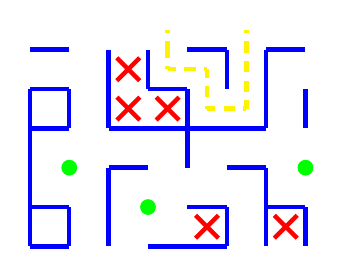
\begin{tikzpicture}[x=0.25cm, y=-0.25cm, ultra thick, blue]
% Walls
    \draw (1,1) -- (3,1);
    \draw (5,1) -- (5,3);
    \draw (5,3) -- (5,5);
    \draw (5,5) -- (7,5);
    \draw (7,5) -- (9,5);
    \draw (9,5) -- (11,5);
    \draw (9,5) -- (9,7);
    \draw (9,3) -- (9,5);
    \draw (7,3) -- (9,3);
    \draw (7,1) -- (7,3);
    \draw (11,5) -- (13,5);
    \draw (13,3) -- (13,5);
    \draw (13,1) -- (15,1);
    \draw (13,1) -- (13,3);
    \draw (9,1) -- (11,1);
    \draw (11,1) -- (11,3);
    \draw (1,3) -- (3,3);
    \draw (1,3) -- (1,5);
    \draw (3,3) -- (3,5);
    \draw (1,5) -- (3,5);
    \draw (1,5) -- (1,7);
    \draw (1,7) -- (1,9);
    \draw (1,9) -- (3,9);
    \draw (1,9) -- (1,11);
    \draw (3,9) -- (3,11);
    \draw (1,11) -- (3,11);
    \draw (15,3) -- (15,5);
    \draw (5,7) -- (7,7);
    \draw (5,7) -- (5,9);
    \draw (5,9) -- (5,11);
    \draw (11,7) -- (13,7);
    \draw (13,7) -- (13,9);
    \draw (13,9) -- (15,9);
    \draw (13,9) -- (13,11);
    \draw (15,9) -- (15,11);
    \draw (9,9) -- (11,9);
    \draw (11,9) -- (11,11);
    \draw (9,11) -- (11,11);
    \draw (7,11) -- (9,11);
% Pillars
    \fill[green] (3,7) circle(0.4);
    \fill[green] (15,7) circle(0.4);
    \fill[green] (7,9) circle(0.4);
% Inner points in accessible cul-de-sacs
    \node at (6,2) {};
    \node at (6,4) {};
    \node at (8,4) {};
    \node at (10,10) {};
    \node at (14,10) {};
% Entry-exit paths without intersections
    \draw[dashed, yellow] (8,1) -- (8,0);
    \draw[dashed, yellow] (8,1) -- (8,2);
    \draw[dashed, yellow] (8,2) -- (9,2);
    \draw[dashed, yellow] (9,2) -- (10,2);
    \draw[dashed, yellow] (10,2) -- (10,3);
    \draw[dashed, yellow] (10,3) -- (10,4);
    \draw[dashed, yellow] (10,4) -- (11,4);
    \draw[dashed, yellow] (11,4) -- (12,4);
    \draw[dashed, yellow] (12,4) -- (12,3);
    \draw[dashed, yellow] (12,3) -- (12,2);
    \draw[dashed, yellow] (12,2) -- (12,1);
    \draw[dashed, yellow] (12,1) -- (12,0);
\end{tikzpicture}
\end{center}
\vspace*{\fill}

\end{document}